% \iffalse
\let\negmedspace\undefined
\let\negthickspace\undefined
\documentclass[journal,12pt,twocolumn]{IEEEtran}
\usepackage{cite}
\usepackage{amsmath,amssymb,amsfonts,amsthm}
\usepackage{algorithmic}
\usepackage{graphicx}
\usepackage{textcomp}
\usepackage{xcolor}
\usepackage{txfonts}
\usepackage{listings}
\usepackage{enumitem}
\usepackage{mathtools}
\usepackage{gensymb}
\usepackage{comment}
\usepackage[breaklinks=true]{hyperref}
\usepackage{tkz-euclide} 
\usepackage{listings}
\usepackage{gvv} 
\usepackage{caption}
\def\inputGnumericTable{}                                 
%\usepackage[latin1]{inputenc}                                
\usepackage{color}                                            
\usepackage{array}                                            
\usepackage{longtable}                                       
\usepackage{calc}                                             
\usepackage{multirow}                                         
\usepackage{hhline}                                           
\usepackage{ifthen}                                           
\usepackage{lscape}

\newtheorem{theorem}{Theorem}[section]
\newtheorem{problem}{Problem}
\newtheorem{proposition}{Proposition}[section]
\newtheorem{lemma}{Lemma}[section]
\newtheorem{corollary}[theorem]{Corollary}
\newtheorem{example}{Example}[section]
\newtheorem{definition}[problem]{Definition}
\newcommand{\BEQA}{\begin{eqnarray}}
\newcommand{\EEQA}{\end{eqnarray}}
\newcommand{\define}{\stackrel{\triangle}{=}}
\theoremstyle{remark}
\newtheorem{rem}{Remark}

\begin{document}

\bibliographystyle{IEEEtran}
\vspace{3cm}

\title{NCERT 12.10 5Q}
\author{EE23BTECH11013 - Avyaaz$^{*}$% <-this % stops a space 
}
\maketitle
\newpage
\bigskip

\renewcommand{\thefigure}{\arabic{figure}}
\renewcommand{\thetable}{\arabic{table}}

\large\textbf{\textsl{Question:}}
In Young’s double-slit experiment using monochromatic light of wavelength $\lambda$, the intensity of light at a point on the screen where path difference is $\lambda$, is $K$ units. What is the intensity of light at a
point where path difference is $\lambda$/3?\\
\large\textbf{\textsl{Solution:}}
\begin{table}[htbp]
\setlength{\extrarowheight}{8pt}
\centering
\begin{tabular}{|c|c|}
\hline 
   \textbf{Parameter}  &\textbf{Description} \\
\hline
     $\lambda$ & Wavelength of monochromatic light\\
\hline
$K$ & Intensity of light at path difference $\lambda$ \\
\hline
$\Delta x$ & Path difference \\
\hline
$A,A_1,A_2$ & Amplitudes of light waves \\
\hline
$\omega$ & Angular frequency \\
\hline
$k$ & Wave number \\ 
\hline
$\phi, \phi_1,\phi_2$ & Phases  \\
\hline
$\Delta \phi $ & Phase differences between two waves \\
\hline
$y_1\brak{t}$ & Displacement produced by $S_1$ \\
\hline
$x_1,x_2$ & Distace travelled by the respective waves \\
\hline
$y_2\brak{t}$ & Displacement produced by $S_2$ \\
\hline
$I_1,I_2,I_{\text{net}},I_{\text{R}}$ & Intensities of coherent waves \\
\hline
\end{tabular}

\caption{Parameters}
\label{tab:parameters}
\end{table}
From \tabref{tab:parameters}:
\begin{align}
%%y\brak{t} &= y_1\brak{t} + y_2\brak{t}  \\
y\brak{t} &= A\sin({2\pi f t - kx_1})  + A\sin({ 2\pi f t - kx_2}) \\
y\brak{t} &=  2A\cos\left(\dfrac{k\Delta x}{2}\right)\sin\left(2\pi f t - \dfrac{k(x_1+x_2)}{2} \right) \label{eq:superposition}
\end{align}
From \tabref{tab:parameters} and equation \eqref{eq:superposition}: 
\begin{align}
\therefore I \propto 4A^2\cos^2\left(\dfrac{k\Delta x}{2}\right)  \label{eq:intensity}
\end{align}
From \tabref{tab:parameters} and equation \eqref{eq:intensity}: 
\begin{align}
 \dfrac{K}{I_r} = \dfrac{4A^2\cos^2\left(\dfrac{2\pi}{2}\right)}{4A^2\cos^2\left(\dfrac{\pi}{3}\right)}
 \implies I_r = \dfrac{K}{4}
 \end{align}
 Hence, the Intensity of light at a point where path difference is $\dfrac{\lambda}{3}$ is $\dfrac{K}{4}$ units.

\begin{table}[htbp]
\centering
\begin{tabular}{|c|c|c|}
    \hline
    \textbf{Parameter} & \textbf{Description} & \textbf{Value} \\
    \hline
     \(x(0)\) & First Term &\(\dfrac{5}{2}\) \\
    \hline
     \(r\) = \(\dfrac{x(1)}{x(0)}\) & Common Ratio & \(\dfrac{1}{2}\) \\
    \hline
      \(x(n)\) & \(n^{th}\) Term & \(\dfrac{5}{2}\left(\dfrac{1}{2}\right)^n \cdot u(n)\) \\
    \hline
     \(x(19)\) & \(20^{th}\) Term &\(\dfrac{5}{2} \left(\dfrac{1}{2}\right)^{19}\) \\
    \hline
     \(u(n)\) &Unit step function & \\
    \hline
  \end{tabular}

\caption{}
\label{tab:intensity}
\end{table}
Assuming $\Delta x= r\lambda$, 

From equation \eqref{eq:intensity}:
\begin{figure}[htbp]
    \centering
    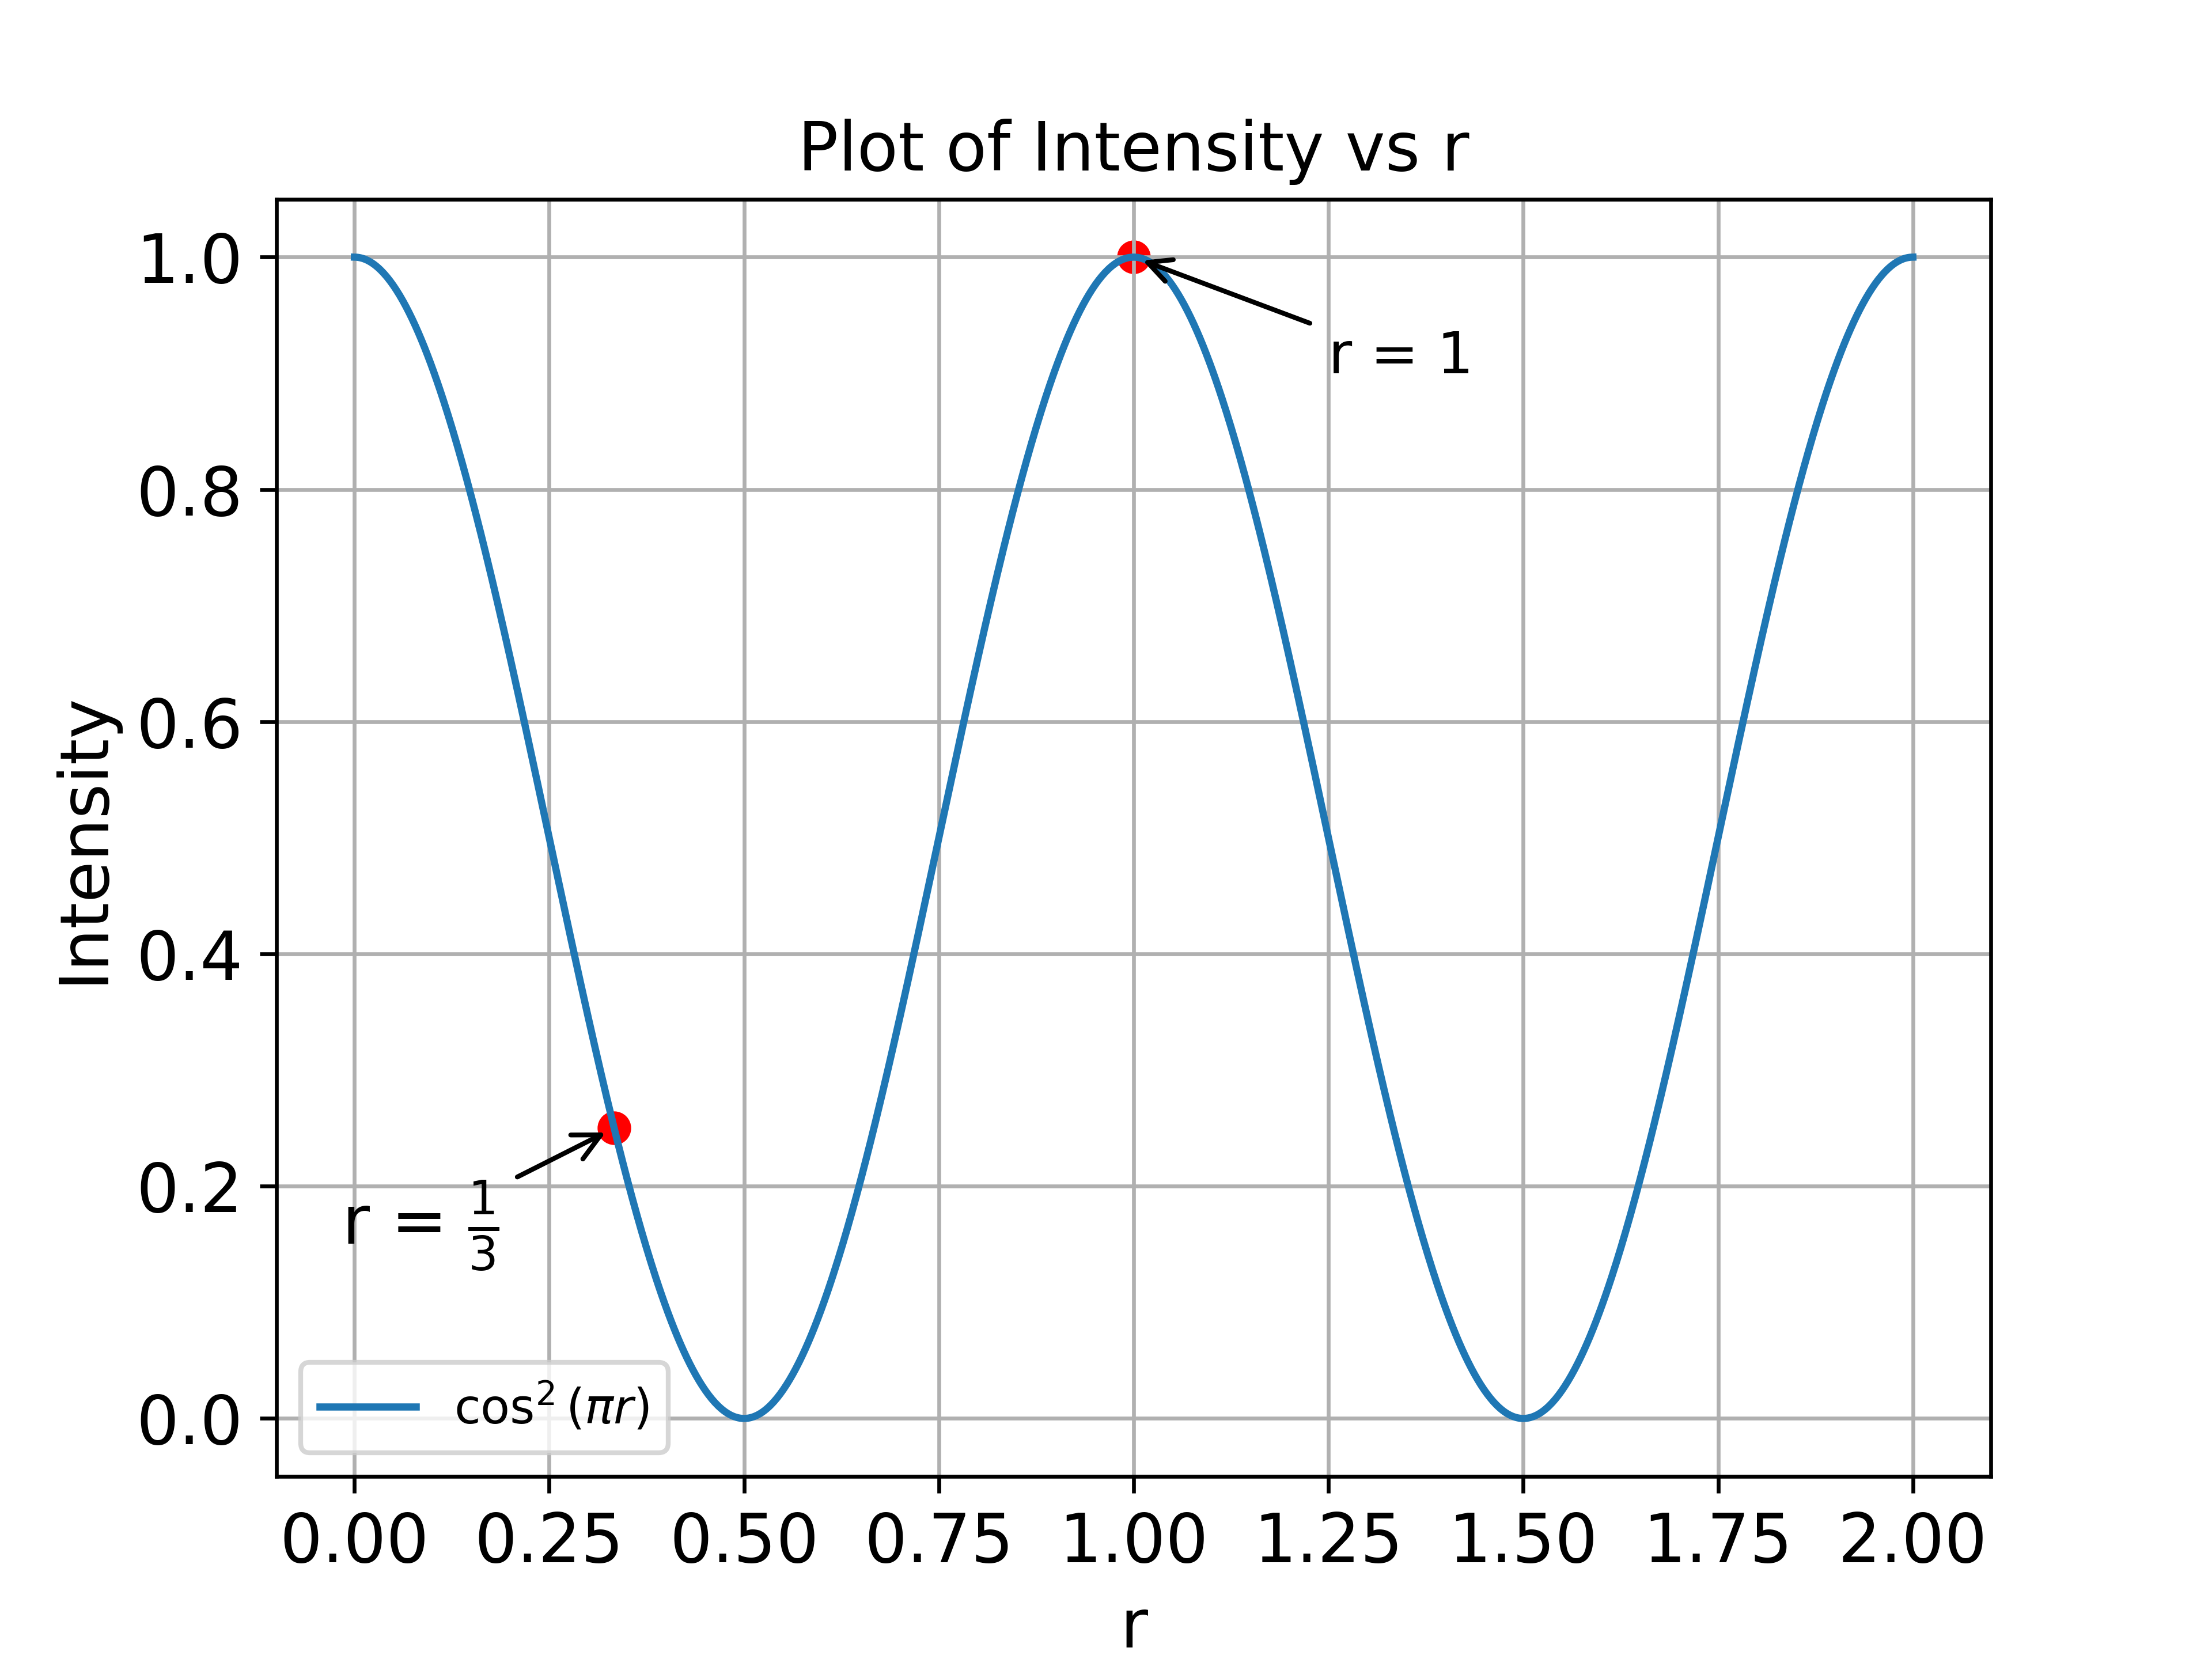
\includegraphics[width = \columnwidth]{figs/intensity_plot.png}
  \caption{}
    \label{fig:graph1}
\end{figure}
\bibliographystyle{IEEEtran}
\end{document}
